\documentclass[t]{beamer}
\usepackage{hyperref}
% Load general definitions
% Preamble file - general definitions, package loading, etc.

%=================================
% Load packages
\usepackage{amssymb,amsmath}
\usepackage{graphicx}
\usepackage{url}
\usepackage{tikz}
\usetikzlibrary{mindmap,trees,arrows}
\usepackage{fancyvrb}
\usepackage[portuguese]{babel} 
\usepackage[utf8]{inputenc}
\usepackage{subfigure}
\usepackage{times}
\usepackage[T1]{fontenc}
\usepackage{cancel}
\usepackage{color}
\usepackage{listings}
\usepackage[document]{ragged2e}

%=================================
% Set mode
\mode<presentation>
{
	\usetheme{Madrid}
	\usecolortheme{structure}
	\useoutertheme{infolines}
	\setbeamercovered{invisible}
}

% Get rid of nav bar
\beamertemplatenavigationsymbolsempty

% Insert frame number at bottom of the page.
\usefoottemplate{\hfil\tiny{\color{black!90}\insertframenumber}} 

%=================================
% Define new commands

\newcommand\Real{{\mathbb{R}}}
%\newcommand{\vi}{\vspace{0.6\baselineskip}}
%\newcommand{\goodgap}{\hspace{\subfigtopskip}\hspace{\subfigbottomskip}}


% Equation environments
\newcommand{\beq}{\begin{equation}}
\newcommand{\eq}{\end{equation}}
\newcommand{\beqs}{\begin{equation*}}
\newcommand{\eqs}{\end{equation*}}
\newcommand{\beqn}{\begin{eqnarray}}
\newcommand{\eqn}{\end{eqnarray}}
% Bold variables
\newcommand{\mbf}[1]{\ensuremath{\mathbf{#1}}}
% Itemization
\newcommand{\bitem}{\begin{itemize}}
\newcommand{\eitem}{\end{itemize}}
\newcommand{\spitem}{\vskip 1em\item}
\newcommand{\bitems}{\begin{itemize}\item}
\newcommand{\benums}{\begin{enumerate}\item}
\newcommand{\eenum}{\end{enumerate}}
% color blocks
\newenvironment{colorblock}[2]{%
\setbeamercolor{block title}{#2}
\begin{block}{#1}}{\end{block}}
% Vertical spacing
\newcommand{\vone}{\vskip 1em}
\newcommand{\vhalf}{\vskip .5em}
% Frame environments
\newenvironment{ftst}[3][t]{%
\begin{frame}{environment=ftst,#1}
\frametitle{#2}
\framesubtitle{#3}}{\end{frame}}
\newenvironment{ftstf}[2]{
\begin{frame}[fragile,environment=ftstf]
\frametitle{#1}
\framesubtitle{#2}}{\end{frame}}
% colors
\definecolor{MyGray}{rgb}{0.5,0.5,0.5}
\definecolor{MyDBGray}{rgb}{0.1,0.1,0.4}
\definecolor{darkgreen}{rgb}{0,0.4,0}
\definecolor{black}{rgb}{0,0,0}
\def\defn#1{{\color{red} #1}}
% Footnote
\renewcommand{\thefootnote}{\alph{footnote}}
% Relaxed footnotes
\newcommand{\lfr}[1]{\let\thefootnote\relax\footnote{\tiny #1}}
% Verbatim environment - using FANCYVRB package
\DefineVerbatimEnvironment%
{rcode}{Verbatim}
{fontsize=\scriptsize}
% Verbatim environment - using LISTINGS package
%\lstnewenvironment{rcode} {\lstset{	language = R,
%									basicstyle = \scriptsize\ttfamily,
%									showspaces = false,
%									showstringspaces = false,
%									showtabs = false,
%									keywordstyle = \color{black}\bfseries,
%									commentstyle = \color{darkgreen},
%									numbers = none,
%									otherkeywords={	<-,
%													ggplot,
%													geom_boxplot,
%													facet_grid,
%													shapiro.test,
%													fligner.test,
%													glht,
%													with},
%									deletekeywords={data,
%													model,
%													residuals,
%													c,
%													axis,
%													default,
%													labels,
%													qq.text}}}%
%{}

% Specific definitions
\title[]{Metodologia Científica}
\subtitle[]{O método científico}
\author[]{Patrícia Lucas\\{\footnotesize }}
\institute{Bacharelado em Sistemas de Informação \\ IFNMG  - Campus Salinas}
\date{\scriptsize Salinas\\Fevereiro 2021}

\begin{document}

% cover page
\setbeamertemplate{footline}{}
\begin{frame}

\begin{center}
\includegraphics[width=.15\textwidth]{}
\end{center}
  \titlepage
  \begin{tikzpicture}[remember picture,overlay]
  \node[anchor=south east,xshift=-5pt,yshift=5pt] at (current page.south east) {\tiny Versão 1.2021};
  \node[anchor=south west,yshift=0pt] at (current page.south west) {
\includegraphics[width=.25\textwidth]{Logos/salinas_horizontal_jpg.jpg}};
  \end{tikzpicture}  
\end{frame}

% Main slides

\begin{ftst}{Referência}{Metodologia Científica}
\vone
\justifying
\begin{figure}
    \centering
    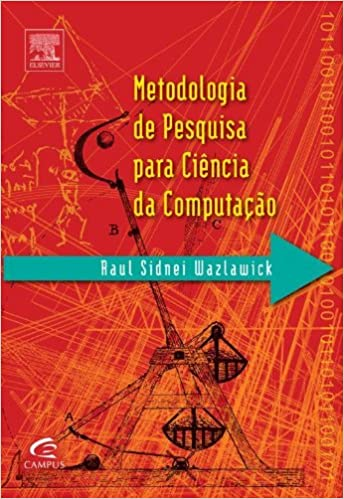
\includegraphics[scale=0.3]{Figuras/ref.jpg}
\end{figure}

WAZLAWICK, R. S. Metodologia de Pesquisa em Ciência da Computação. Rio de Janeiro: Campus, 2009.

\end{ftst}

%=====

\begin{ftst}{Como a ciência funciona?}{Método científico}
\justifying
\small
\begin{itemize}
    \item O método científico é tradicionalmente apresentado no primeiro capítulo dos livros didáticos como uma receita simples para a realização de investigações científicas. 
    \item Embora muitos pontos úteis estejam incorporados neste método, ele pode ser facilmente mal interpretado como linear e "livro de receitas":
\begin{figure}
    \centering
    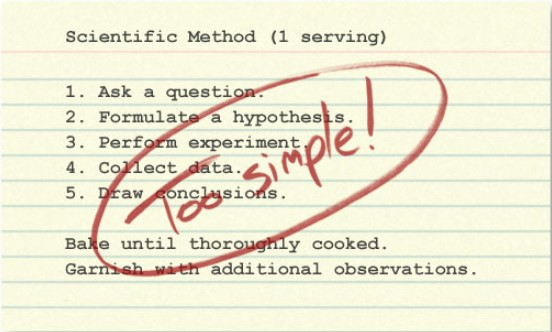
\includegraphics[scale=0.4]{Figuras/receitas.jpg}
\end{figure}
    \item Esta versão do método científico é tão simplificada e rígida que falha em retratar com precisão como a ciência real funciona.
\end{itemize}
\end{ftst}

%=====

\begin{ftst}{Como a ciência funciona?}{Método científico}
\justifying
\small
\textcolor{blue}{O método científico simplificado e linear implica que os estudos científicos seguem uma receita linear invariável.}
\vone
Mas, na realidade, os cientistas se envolvem em muitas atividades diferentes em muitas sequências diferentes. As investigações científicas geralmente envolvem a repetição dos mesmos passos, muitas vezes, para dar conta de novas informações e ideias.
\vone
\vone
\textcolor{blue}{O método científico simplificado e linear implica que a ciência é feita por cientistas individuais trabalhando por meio dessas etapas isoladamente.}
\vone
Mas, na realidade, a ciência depende de interações dentro da comunidade científica. Partes diferentes do processo da ciência podem ser realizadas por pessoas diferentes em momentos diferentes.

\end{ftst}

%=====

\begin{ftst}{Como a ciência funciona?}{Método científico}
\justifying
\small

\textcolor{blue}{O método científico simplificado e linear implica que a ciência tem pouco espaço para criatividade.}
\vone
Mas, na realidade, o processo da ciência é emocionante, dinâmico e imprevisível. 
\vone
\vone
\textcolor{blue}{O método científico simplificado e linear implica que a ciência conclui.}
\vone
Mas, na realidade, as conclusões científicas são sempre revisáveis se garantidas pelas evidências. As investigações científicas estão frequentemente em andamento, levantando novas questões, mesmo quando as antigas são respondidas.
\end{ftst}


%=====

\begin{ftst}{O verdadeiro processo da ciência}{Método científico}
\justifying
\small

\textcolor{blue}{O processo da ciência é iterativo:}
\vone
a ciência gira em torno de si mesma para que ideias úteis sejam construídas e usadas para aprender ainda mais sobre o mundo natural. Isso geralmente significa que investigações sucessivas de um tópico levam de volta à mesma pergunta, mas em níveis cada vez mais profundos.
\vone
\vone
\textcolor{blue}{O processo da ciência não é predeterminado:}
\vone
Qualquer ponto no processo leva a muitas próximas etapas possíveis, e onde essa próxima etapa leva pode ser uma surpresa.

\end{ftst}

%=====

\begin{ftst}{Classificação da ciência}{Método científico}

A complexidade do universo e a diversidade de fenômenos que nele se manifestam, aliadas à necessidade do homem de estudá-los para poder entendê-los e explicá-los, levaram ao surgimento de diversos ramos de estudo e ciências específicas.

\begin{figure}
    \centering
    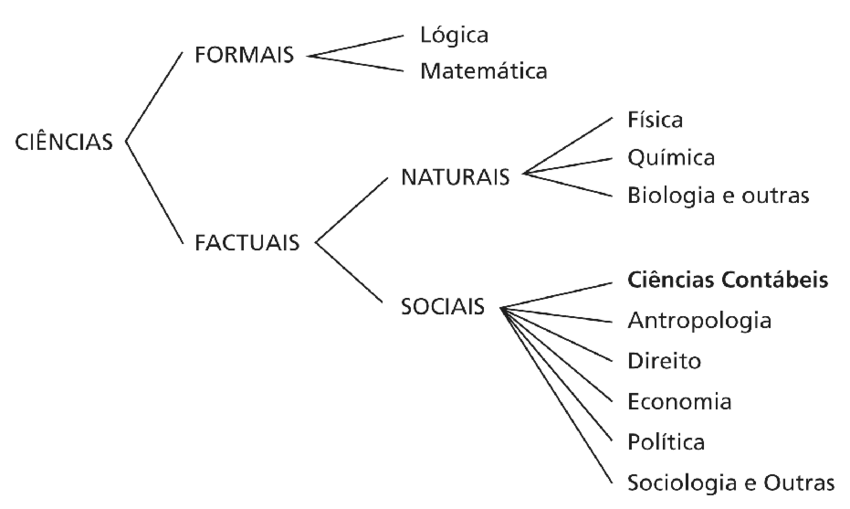
\includegraphics[scale=0.25]{Figuras/01_classificacao_ciencia.png}
    \label{fig:classificacao_ciencia}
\end{figure}

\scriptsize
Tabela de classificação das áreas de conhecimento de acordo com a CAPES: \href{http://lattes.cnpq.br/documents/11871/24930/TabeladeAreasdoConhecimento.pdf/d192ff6b-3e0a-4074-a74d-c280521bd5f7}{\textcolor{green}{clique aqui.}}

\end{ftst}

%=====


\begin{ftst}{Classificação da ciência}{Método científico}
\justifying
Outra classificação das ciências deriva da forma como seus estudos são aplicados, como as ciência puras e aplicadas.
\vone
\textbf{Ciência pura:} estudam os conceitos básicos do conhecimento sem preocupação com sua imediata aplicação.
\vone
\textbf{Ciências aplicadas:} visam à realização de descobertas que possam ser imediatamente aplicadas a algum processo industrial ou assemelhado para produzir algum tipo de ganho.

\end{ftst}

%=====

\begin{ftst}{Classificação da ciência}{Método científico}
\justifying
Outra classificação caracteriza as ciências em exatas e inexatas:
\vone
\textbf{Ciências exatas:} são aquelas cujos resultados são precisos. Suas leis são altamente preditivas e previsíveis. Experimentos podem ser repetidos inúmeras vezes, produzindo o mesmo resultado ou resultados estatisticamente previsíveis. São classificadas entre as ciências exatas a matemática, por excelência, mas também a física, a química e partes de algumas ciências naturais e sociais.
\vone
\textbf{Ciências inexatas:}  são aquelas que podem prever comportamentos gerais de seus fenômenos, mas cujos resultados nem sempre são os esperados. Isso usualmente ocorre porque é muito difícil avaliar todos os dados que produzem os resultados. Entre as ciências inexatas pode-se incluir a meteorologia, a economia e a maioria das ciências sociais.

\end{ftst}

%=====




\begin{ftst}{Conceito de método}{Método científico}
\vone
\justifying
As ciências caracterizam-se pela utilização de métodos científicos, mas nem todos os ramos de estudo que empregam esses métodos são ciências. A utilização de métodos científicos não é, portanto, da alçada exclusiva da ciência, mas não há ciência sem o emprego de métodos científicos.\\ \vone

"\textbf{Método} é o conjunto das atividades sistemáticas e racionais que, com maior segurança e economia, permite alcançar o objetivo de produzir conhecimentos válidos e verdadeiros, traçando o caminho a ser seguido, detectando erros e auxiliando as decisões do cientista".

\end{ftst}

%=====

\begin{ftst}{O método científico}{Método científico}
\justifying
\textcolor{blue}{"O método científico é a teoria da investigação".}
\vone
O método científico é particularmente importante em computação porque, como ciência, ela não pode se ocupar apenas da coleta de dados. A explicação dos dados é muito mais importante.
\vone
\footnotesize
Um aluno aplicou um questionário a cinco pessoas para uma pesquisa de opinião eleitoral. Três responderam “Candidato A”, e duas, “Candidato B”. O aluno concluiu que
havia uma tendência para o “A” (60\% de respostas “A”). Mas que valor tem essa conclusão? 

\end{ftst}

%=====

\begin{ftst}{O método científico}{Método científico}
\justifying

\footnotesize
Se um grupo usou um software educacional e outro não, e o grupo do software educacional foi melhor na avaliação, isso prova o quê? Pode ser que o software tenha melhorado a aprendizagem? Sim. Mas também pode ser que os alunos que usaram o software simplesmente tenham estudado mais por vergonha de tirarem notas mais baixas que os outros que não usaram o software. Pode ser também que o grupo que não usou o software se sentiu desprestigiado e se interessou menos pelo assunto. Ou seja, várias explicações podem existir. Cabe ao pesquisador descobrir a mais provável de acordo com o método científico.

\end{ftst}

%=====

\begin{ftst}{Empirismo}{Método científico}
\vone
\justifying
O \textbf{empirismo} estabelece que toda teoria científica deve ser baseada em observações que podem ser testadas e produzir leis gerais com poder preditivo. Dessa forma, teorias científicas podem ser verificadas à luz da evidência empírica e, quando não explicam adequadamente os fatos observáveis, podem ser refutadas.
\vone
\footnotesize
Um aluno escreveu logo no início de seu artigo: “O interesse pela internet vem crescendo muito ao longo dos últimos anos.”
Mas isso tem base empírica ou é apenas uma sensação dele? Será verdade? Quem disse? Como ele observou esse fato? Essa
simples informação possivelmente até é verdadeira, mas quem publicou? Quais são os dados objetivos, ou seja, os números?
Será essa afirmação ainda verdadeira hoje? Não estará o interesse pela internet estável ou diminuindo neste momento?
O leitor provavelmente responderá “claro que não” a esta última pergunta. Mas como pode ter tanta certeza? Tem dados?
\end{ftst}

%=====

\begin{ftst}{Positivismo}{Método científico}
\vone
\justifying
O \textbf{positivismo} propõe que a ciência deva se basear apenas em valores humanos, deixando a teologia, o misticismo e a metafísica em outra esfera que não deve interferir nas observações e teorias científicas.
\vone
A ciência não nega categoricamente a maioria das crenças populares, religiosas ou não. Mas, enquanto tais crenças não
forem testadas pelo método científico, ela nada pode afirmar sobre elas.


\end{ftst}

%=====

\begin{ftst}{Pragmatismo}{Método científico}
\vone
\justifying
O \textbf{pragmatismo} é uma corrente filosófica que se contrapõe ao realismo científico. Os realistas defendem que a ciência de
fato descreve a realidade. Já os pragmáticos assumem que não é possível saber exatamente o que seja a realidade e que, assim, a ciência explica apenas os fenômenos observados, e suas previsões são consistentes e úteis.
\vone
De acordo com o pragmatismo, a ciência não faz declarações sobre a natureza como ela é, mas sobre nossas observações a respeito
da natureza.


\end{ftst}

%=====

\begin{ftst}{Objetividade}{Método científico}
\vone
\justifying
Outra característica patente do método científico é a \textbf{objetividade}, ou seja, a possibilidade de que duas pessoas quaisquer com nível aceitável de competência possam chegar às mesmas conclusões ao analisarem os dados.
\vone
O critério de objetividade coloca de lado, então, as opiniões em ciência porque opiniões são subjetivas e dependem da experiência, caráter e motivação das pessoas que as emitem.


\end{ftst}

%=====

\begin{ftst}{Objetividade}{Método científico}
\vone
\justifying
Qualquer observação ou grandeza que se queira avaliar deve ser definida de forma que
leituras possam ser feitas independentemente do observador que as toma.
\vone
Por exemplo, o pesquisador poderia dizer que um sistema é “fácil de usar” se determinado conjunto de tarefas predefinido puder ser executado por um usuário com determinado grau de treinamento dentro de um período de tempo predeterminado. 


\end{ftst}

%=====


\begin{ftst}{Indução}{Método científico}
\vone
\justifying
O método científico também apresenta como um de seus princípios que uma situação que se sustenta em todos os casos observados se sustenta em todos os casos, até prova em contrário. Isso é conhecido como \textbf{princípio da indução}.
\vone



\end{ftst}

%=====

\begin{ftst}{Refutação}{Método científico}
\vone
\justifying
O \textbf{princípio da refutação} ou contradição de uma teoria estabelece que qualquer teoria científica que procura explicar fatos observáveis está sempre aberta para ser invalidada, caso não seja capaz de explicar novos observáveis.
\vone



\end{ftst}

%=====

\begin{ftst}{Coerentismo}{Método científico}
\vone
\justifying
O \textbf{princípio do coerentismo} está altamente ligado com a filosofia do pragmatismo. 
\vone
Então, em nenhum momento o cientista vai afirmar que sua teoria explica a realidade. Ele só pode afirmar que sua teoria é coerente com as observações e que, pelo princípio da indução, na falta de refutação essa teoria pode ser aceita como explicação.

\end{ftst}

%=====

\begin{ftst}{Lâmina de Occam}{Método científico}
\vone
\justifying
O \textbf{princípio da lâmina de Occam} diz que, no caso de várias teorias que explicam as mesmas observações, deve-se preferir a mais simples dentre elas.
\vone
O termo "lâmina" sugere que, com o uso da parcimônia, a hipótese mais complicada é “cortada”. 

\end{ftst}

%=====




\end{document}